
\lstset{
	backgroundcolor=\color{lbcolor},
	tabsize=2,
	rulecolor=,
	language=matlab,
        basicstyle=\tiny,
        upquote=true,
        aboveskip={1\baselineskip},
        columns=fixed,
        showstringspaces=false,
        extendedchars=true,
        breaklines=true,
        prebreak = \raisebox{0ex}[0ex][0ex]{\ensuremath{\hookleftarrow}},
        frame=single,
        showtabs=false,
        showspaces=false,
        showstringspaces=false,
        identifierstyle=\ttfamily,
        keywordstyle=\color[rgb]{0,0,1},
        commentstyle=\color[rgb]{0.133,0.545,0.133},
        stringstyle=\color[rgb]{0.627,0.126,0.941},
		numbers=left,
}


\begin{figure}[t]
\lstset{language=C,numbersep=4pt}
\begin{center}
\begin{lstlisting}
	for(int i =0 ; i < 100000; i++)
		a[i] = c[i]*b[i];
	
\end{lstlisting}
\end{center}
\vspace{-1em}
\captionof{lstlisting}{Example of small loop.}
\label{lst:basic}
\vspace{-1em}
\end{figure}

\begin{figure}[t]
    \centering
    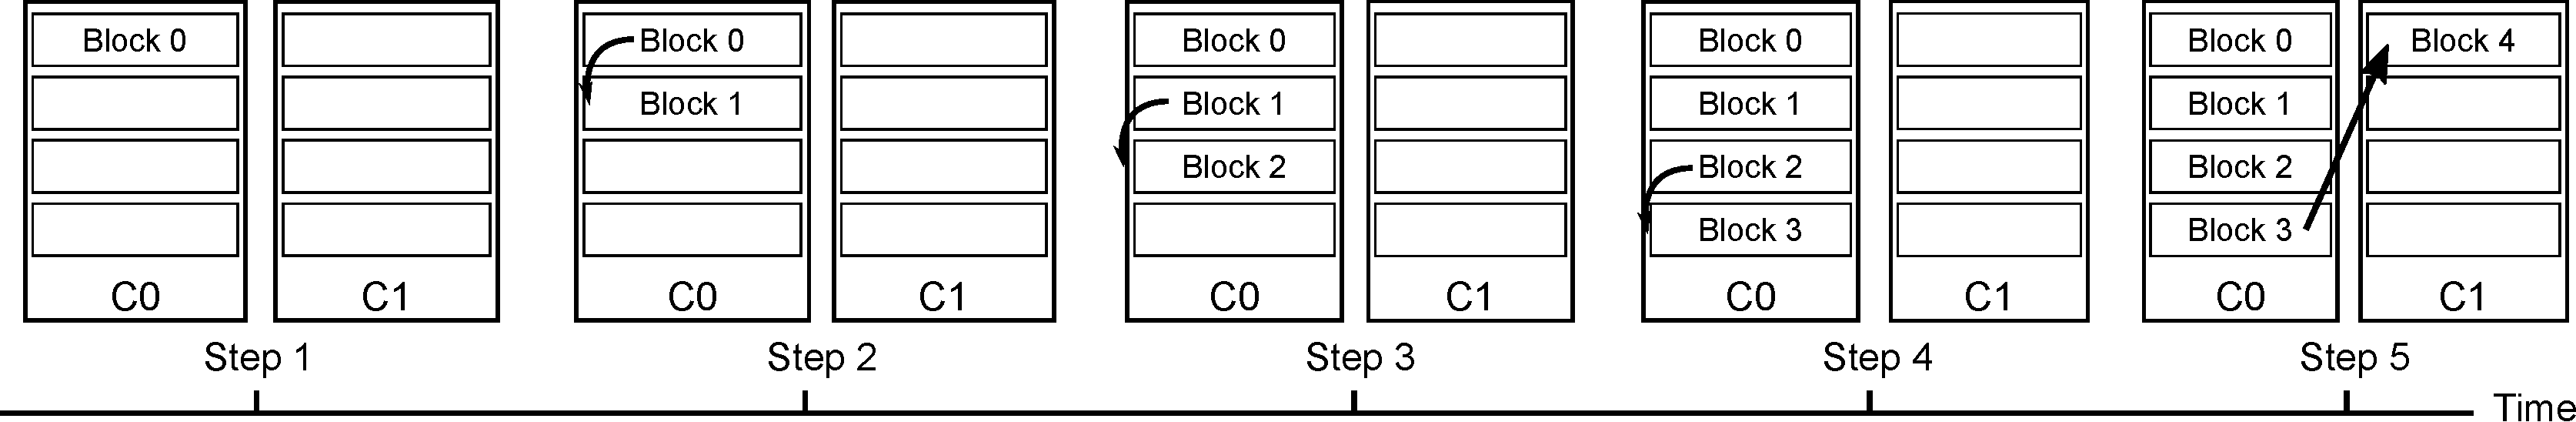
\includegraphics[width=1\textwidth]{chapter3/graphics/normfetch.pdf}
    \caption{Example of the current fetching model on a 2 core composition. Each core has 4 segments, the arrows represent the block generating the predictions.}
    \label{fig:old_fetch}
\vspace{1em}
%\end{figure}
%\begin{figure}[t]
    \centering
    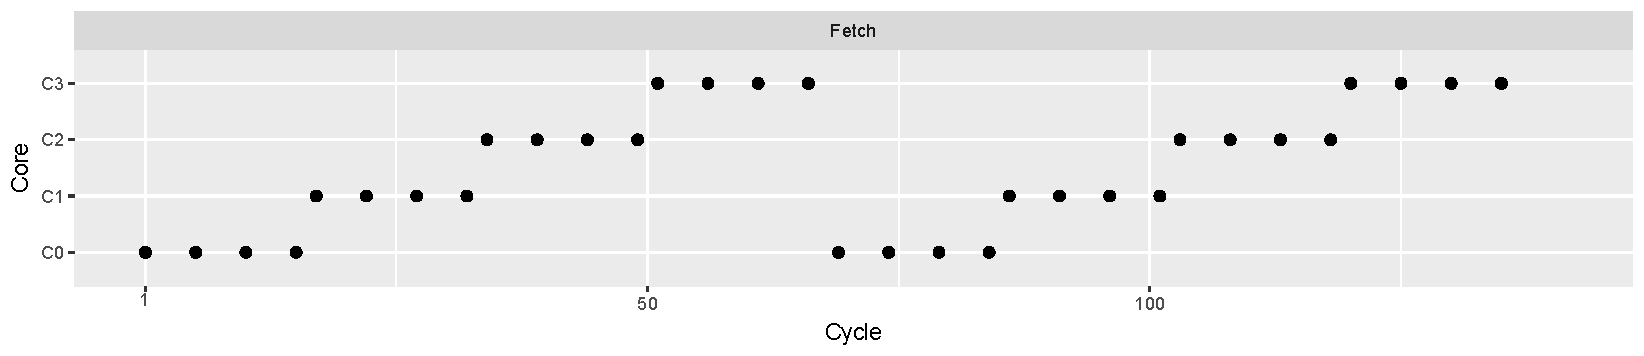
\includegraphics[width=1\textwidth]{chapter3/graphics/4fetchnorm2.pdf}
    \caption{Trace of when cores fetch blocks when executing Listing~\ref{lst:basic} on a 4 core composition. Y axis represents a core in the composition, X axis represents time.}
    \label{fig:fetch_norm}
\vspace{1em}
\end{figure}
\subsection{Current fetching scheme}
	
The current block fetching scheme, Serial Fetch (SF) requires that a core fills its instruction window before another core in the composition can fetch a block.
Figure~\ref{fig:old_fetch} illustrates how a two core composition fetches blocks in SF when blocks only take up a single lane of the instruction window.
Once Core 0 is full, it submits a fetch request to Core 1 as seen in Figure~\ref{fig:old_fetch} and stops fetching.
As the figure shows, Core 1 is not active until the 5th fetch request.

The main issue with the SF scheme is that cores in a composition depend on each other in order to fetch blocks.
For example, if Listing~\ref{lst:basic} is compiled without unrolling and executed on a 4 core composition, each core would have to fetch 4 iterations of the loop before sending the next fetch request to another core.
To illustrate how fetching can be a bottleneck in this situation, instrumentation was added to the simulator to track when cores fetch blocks in order to be able to visualise how long it takes to fill up a core composition.
Figure~\ref{fig:fetch_norm} plots the when cores fetch blocks for a 4 core composition executing the code in Listing~\ref{lst:basic}.
Each point represents a block fetch, the X-axis represents the time (in cycles) whilst the Y axis represents which core has started fetching a block.
The figure shows that there are 50 cycles between the first block fetched by Core 0 and the first block fetched by Core 3.
Given that a block in Listing~\ref{lst:basic} takes only 10 cycles to execute, this means that Core 0 is inactive when Core 3 fetches.
This is due to the fact that once Core 0 submits a fetch request to Core 1, it will have to wait for Core 3 to send it a fetch request.

Having a serialised block fetching scheme for core composition is one of the main bottlenecks for performance when the compiler cannot produce large blocks.
This means that core composition is not an efficient method of executing small blocks in parallel, compared to using multithreading.
When using multithreading cores can fetch blocks independently and thus maximize throughput easily, the size of the block will not have the same impact on performance.
A mechanism that can alleviate communication between cores is a first step in improving block throughput for core-compositions.

\subsection{Round Robin Fetching Scheme}

Fetching blocks in a serial fashion currently makes large core compositions more difficult to use efficiently when blocks are small.
Whilst serialising fetches aims to improve the efficiency of a single core by ensuring that its instruction window is full, it makes populating large core compositions a challenging task.
If cores can fetch blocks independently, this allows larger core compositions to populate cores in a much quicker fashion.

This section demonstrates how the fetching mechanism can be modified to allow for cores to fetch blocks in parallel.
It starts with a generalised version of the fetching algorith for \textit{n} cores in a composition.
This is followed by a more in-detail example using a two core composition.
Finally it compares the performance of the new fetching scheme with the current fetching scheme on a synthetic benchmark.

\subsubsection{Generalised form}
The advantage of core composition is that multiple cores can execute the same thread.
Thus, the fact that the SF scheme prioritises filling a single core before using another core in the composition is counter-intuitive as it reduces the chance that all the cores are in use.
The new fetching scheme has two design objectives: reduce communication amongst cores and ensure that each core in the composition is always executing at least one block.
Sequential blocks should not be found on the same core, instead they should all be on separate cores and fetched in a round robin fashion.
This ensures a more equal distribution of work amongst all the cores in the composition, and also reduces the overhead of ensuring each core has a block.

Currently, if a core does not have a block in its instruction window, it waits until another core in the composition sends it a fetch request.
If blocks are distributed equally amongst all cores using a round robin model, this new model still requires that each core must submit a fetch request to the next core.
This means that changing the fetching scheme to a round robin scheme does not suffice to reduce communication amongst cores.
However, once a core has a block it can use branch prediction to predict the next block it must fetch, rather than waiting for another fetch request from a core.
As this new fetching mechanism employs a round robin scheme, the branch predictor should predict a block that is multiple steps into the future rather than the immediate branch.
By allowing cores to fetch blocks in \textit{strides}, instead of sequentially, the new fetching mechanism not only ensures cores have an equal amount of work, but that they can fetch in parallel.

\begin{algorithm}

\textbf{n} = Number of cores in the composition\\
\textbf{Composition[n]} = Core Composition Array\\
\textbf{branches[2]} = Branch Predictions for current block\\

\While{Program is Executing}
{
\Comment{Do branch prediction for up to 2 blocks}
branches = prediction[i+1, i+n]\\
\Comment{If the predictor generated 2 predictions}
\eIf{size(branches) == 2}
{
\Comment{If next core in composition is empty submit block i + 1 to it}
	\eIf{empty(Composition[currentPosition+1])}
	{
		submitToNextCore(branches[0])\\
		
		\eIf{myCore.full() == false}
		{
			submitToMyself(branches[1])
		}
		{
			buffer.push(branches[1])\\
		}
	}
	{
	\eIf{myCore.full() == false}
	{
		submitToMyself(branches[1])\\
	}
	{
		buffer.push(branches[1])\\
	}
	
	}
}
{
\Comment{If only block i + 1 prediction is valid}
	\If{empty(Composition[currentPosition+1])}
	{
		submitToNextCore(branches[0])\\
	}
}	
}
\caption{Overview of fetching algorithm for \textit{n} cores fused}~\label{alg:fetch}
\end{algorithm}

\begin{algorithm}
\textbf{n} = Number of cores in the composition\\
\textbf{Composition[n]} = Core Composition Array\\

\While{Program is Executing}
{
	\If{block is committing}
	{
		Composition[currentPosition+1] = Non Speculative\;
	}
	\If{not IsBlockRunning(Composition[currentPosition+1], block+1)}
	{
		submitToNextCore(block+1 PC)
	}
	
	\If{buffer.size() \textgreater{} 0}
	{
		fetch(buffer[0])
		buffer.pop()
	}
	\Else
	{
		Idle
	}
}
\caption{Overview of commit stage for \textit{n} cores fused}~\label{alg:commit}
\end{algorithm}

Algorithm~\ref{alg:fetch} explains how the new fetching scheme, named Round Robin Fetch (RRF) works for \textit{n} cores in a composition.
In the general case, when a core composition is created, each core, aside from the core that initiated the composition, is empty.
When a core fetches a $block_i$, if the next core is empty, it makes two branch predictions, one for $block_{i+1}$ and one for $block_{i+n}$.
The predictions do not have to be done on the same cycle, however previous work on multi-block ahead branch predictors demonstrated that two predictions per cycle is possible~\cite{SeznecMultipleBlock}.
The core submits a fetch request to the next core in the composition for $block_{i+1}$ and then uses the prediction $block_{i+n}$ to fetch its next block.
If the next core is not empty, then the current core simply predicts $block_{i+n}$.

In case that a core cannot predict $block_{i+n}$, it simply submits a prediction for $block_{i+1}$ to the next core.
The core will then have to wait for another core in the composition to send it the prediction for $block_{i+n}$.
Whilst this case may impact overall throughput, it is no different than the SF scheme as SF would also stop fetching after $block_{i+n-1}$ and wait for $block_{i+n}$'s PC to be resolved.

In the SF scheme, when a core is full, it submits a fetch request to another core in the composition by sending the address of a block to a buffer found on that core.
To ensure cores are always fetching blocks in RRF, the buffer is used when a core has filled up its instruction window and can no longer fetch blocks.
Instead of sending the fetch request to another core, a core saves the block address in its own buffer, and will handle that fetch request once it has committed a block.
In this chapter, a core can only have one buffered PC at a time.

Algorithm~\ref{alg:commit} shows how blocks are committed in RRF.
When committing $block_i$, the core sets the next core in line to be the non-speculative core.
This is due to the fact that the next core in line will always have $block_i+1$.
If the next core in line does not yet have $block_{i+1}$ due to no prediction having been made, then the committing core will submit the resolved PC to the next core, rather than fetching it for itself.
As previously stated, if the core has a PC in its buffer, it immediately starts fetching a new block.
However, if it has no PC in its buffer, it must wait on another core to send it a request.
\subsubsection{Two core example}
	
\begin{figure}[t]
    \centering
    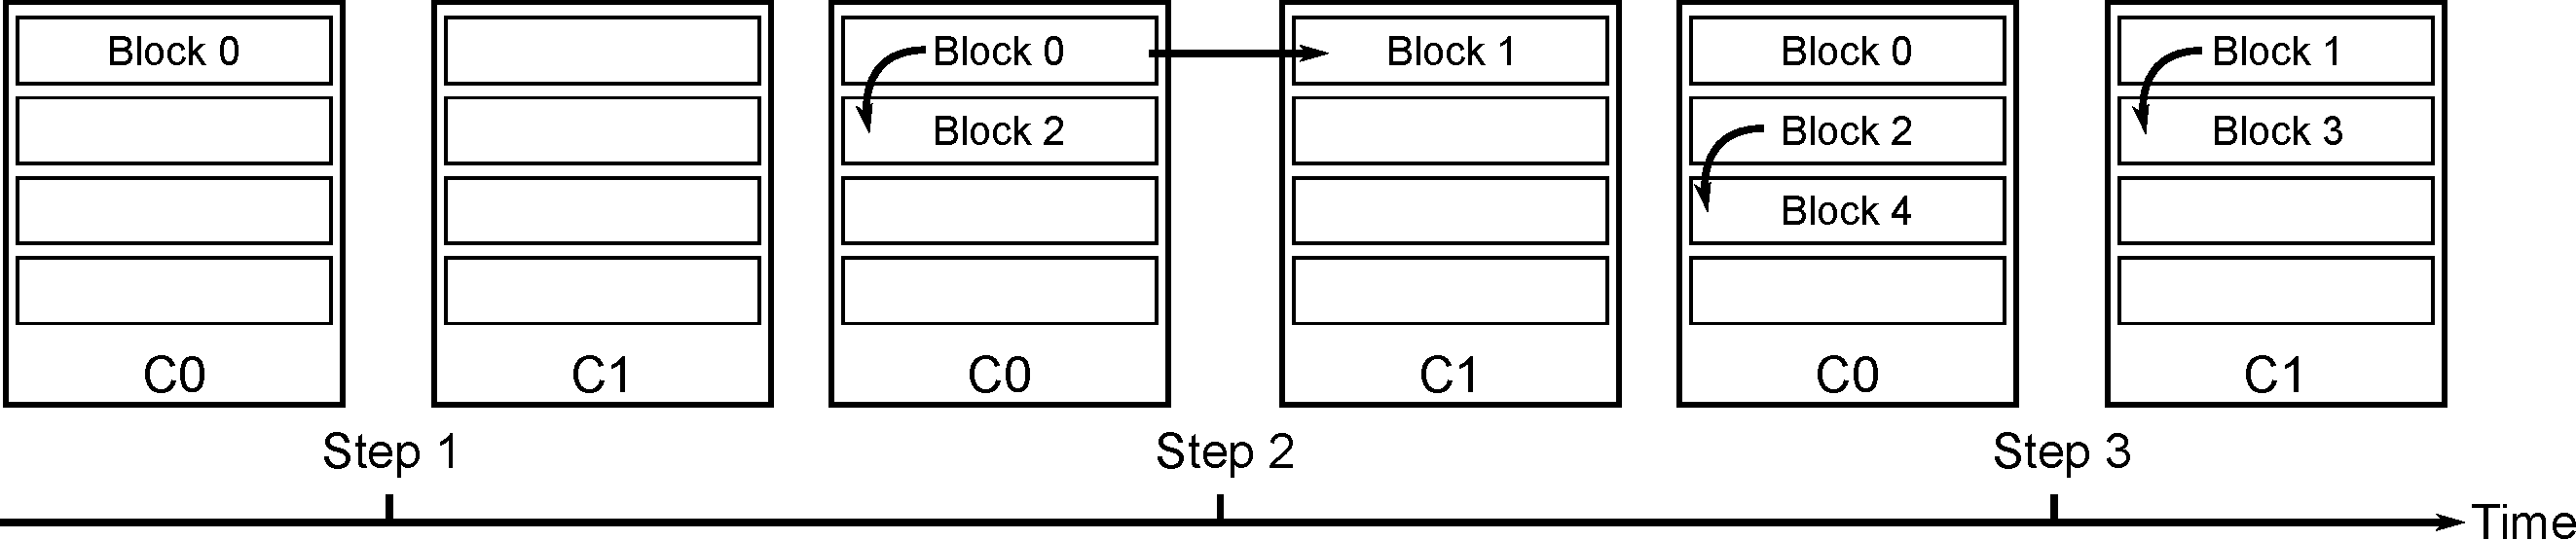
\includegraphics[width=1\textwidth]{chapter3/graphics/fetching-model.pdf}

    \caption{Example of RRF on a 2 core composition. Each core has 4 segments, the arrows represent the block generating the predictions. This figure shows the first 3 steps of a new core composition fetching blocks.}
    \label{fig:new_fetch_ex}
\vspace{1em}
	\end{figure}
%Given a 2 core-fusion \{$Core_0$,$Core_1$\} using a ITTAGE~\cite{SeznecITTAGE} multi-block ahead branch predictor described by A. Seznec et al in~\cite{SeseznecMultipleBlock} the cores can make two predictions in a single cycle: one for itself and one for the next core.
Figure~\ref{fig:new_fetch_ex} gives an overview of the first few cycles of using RRF with two cores fused.
When $Core_0$ starts the composition and fetches the first block, $block_0$, if it is able to predict $block_2$ is will submit a fetch request for $block_1$ on $Core_1$ whilst also attempting to fetch $block_2$ for itself.
On the next cycl	e $Core_1$ receives the request for $block_1$ and starts fetching the block.
Once $Core_1$ can make a branch prediction it will attempt to predict for $block_3$ instead of $block_2$; this is because $block_2$ was already predicted and fetched on $Core_0$.

%In this new fetch mechanism, when a core is in fetching mode, it does not attempt to predict $block_{n+1}$ but rather $block_{n+numberOfCoresInComposition}$; the reason behind this will be clarified shortly.
%If $Core_0$ or $Core_1$ attempts to fetch a block when it is full, it can submit the new block's PC to a buffer; the core then stops attempting to allocate new blocks.
%Once the full Core has committed a block, it checks if it has a buffered PC, and if it does it fetches that block.

%As long as $Core_0$ and $Core_1$ can fetch and predict blocks correctly, they will fetch in a pipelined fashion.
%This means that $Core_0$ will have blocks \{0,2,4,6\} whilst $Core_1$ has \{1,3,5,7\}.
%The reason behind this is to minimize the Synchronization Cost defined in Chapter 2 as now each Core will be committing a block in turn.

%In the case that $Core_0$ cannot make a prediction for $block_2$ it will only send a fetch request for $block_1$ to $Core_1$.
%When this happens, $Core_0$ will no longer be able to fetch blocks until it is sent a PC from $Core_1$.
%The request will happen once $Core_1$ commits $block_1$ and the PC of $block_2$ is resolved.
%Whilst this case may impact overall throughput, it is no different than the current model as the current model would also stop fetching after $block_1$ and wait for $block_2$'s PC to be resolved.

\subsubsection{Limitations}

Whilst RRF allows for cores to fetch out of order in parallel, blocks must still be dispatched in order.
This is to ensure that blocks do not execute data-dependent register reads out of order, when dependencies are not yet determined.
To achieve this, a record of the last dispatched block number is kept in a shared counter.
When a block tries to dispatch instructions it checks the counter, if its block number is sequentially next then it atomically updates the counter to the value of its block number and dispatches its block.

This mainly impacts the performance of large compositions when the system is not in a steady-state of fetching and dispatching blocks and the blocks are small.
This is due to the fact that the fetch stride is larger and thus cores will have to wait longer for blocks on other cores to dispatch.
For example, when starting a composition of 16 cores, the first core will have blocks 1 and 17 in its instruction window.
However, it will have to wait on all other cores to fetch a block before dispatching block 17, which may take 60 or more cycles.

This limitation could be alleviated by creating a more complex fetching scheme that takes into account which cores are available to fetch and dispatch blocks immediately, rather than having a stride that is fixed ahead of time.
Such a scheme may require to centralise the fetching though, as it would require more awareness of what each core is executing.
This is not explored throughout this Chapter, yet it is suggested as future work.

\subsection{Evaluating the round robin fetch scheme on a synthetic block}

\begin{figure}[t]
    \centering
    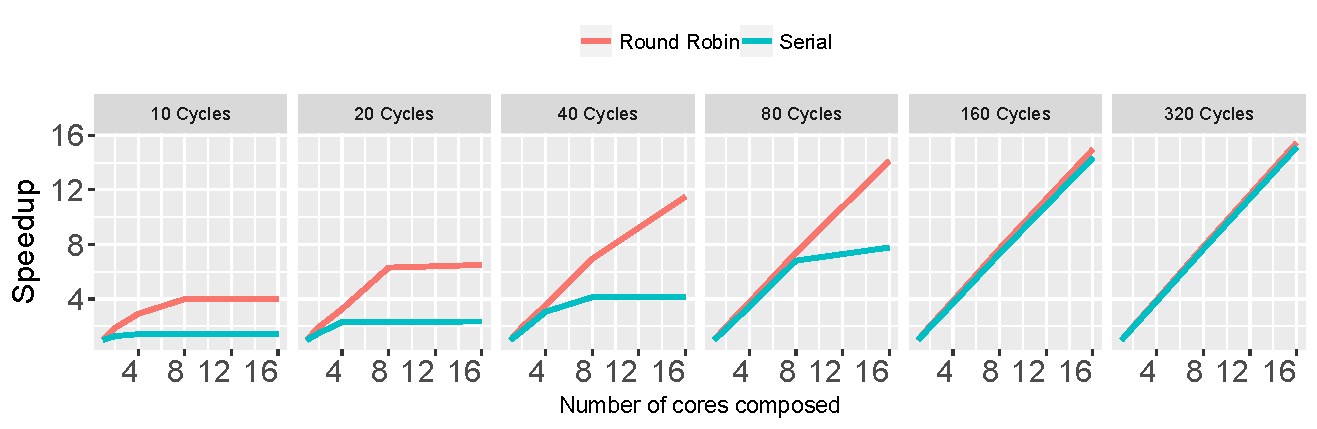
\includegraphics[width=1\textwidth]{chapter3/graphics/motivation_fetch.pdf}
    \caption{Speedup obtained when executing the synthetic block with varying execution times (facets) with the current fetching technique and new fetching technique. Higher is better.}
    \label{fig:new_fetch_ex}
\vspace{1em}
\end{figure}

Before evaluating the performance of RRF on a set of benchmarks, it is important to measure the potential performance increase on a simpler case.
This is due to the fact that other factors than the size of blocks, such as data-dependencies, cache misses or load-store queue violations can affect the performance of a composition.
Therefore, evaluating the new fetching scheme on a synthetic benchmark can provide a ceiling for the maximum performance gains when using RRF.

For this section the synthetic block is only four instructions long using a custom instruction whose execution time is defined ahead of the simulation.
The reason a four instruction block was chosen is due to the fact that it allows for four blocks to be fetched on each core, which is the worst-case scenario for the SF scheme.
Whilst the SF scheme is susceptible to small blocks, the main issue is when these blocks execute quickly, as it means that the composition cannot be filled.
On the other hand, if a block is small yet hundres of cycles to execute, for example due to multiple cache misses, then the SF scheme would still perform fine, as filling cores would take less time than executing blocks.
This is why the execution time of the block is variable, as it allows to cover different cases.
For this experiment, six different execution times are explored: $Exec=\{10,20,40,80,160,320\}$.

Figure~\ref{fig:new_fetch_ex} shows the speedup obtained when using core composition when executing the synthetic benchmark, with the SF or RRF scheme.
The baseline in this case is a single core executing the benchmark.
The facets represent one of the different execution times of the block whilst the colours represent the different fetching schemes.
The results in the figure show that unless a block is at least 80 cycles long, it is difficult to efficiently use 16 core compositions using the normal fetching scheme.
To give a point of reference -- using data gathered from the SD-VBS benchmarks from Chapter~\ref{chp:cases} -- the average execution time of a block in SD-VBS is 20 cycles long.
However, with the new fetching scheme, 16 cores becomes useful when blocks are at least 40 cycles long, enabling a 3x speedup compared to the old fetching scheme.
For smaller core compositions, such as 2 and 4 fused cores, using a different fetching scheme from the traditional method allows for core composition to speedup execution when blocks are even 10 cycles long.
